\lecture{8}{2025-02-12}{Suite d'élément de $\mathbb{R}^n$}{}

\begin{parag}{Rappel: Sous-ensembles ouvert et fermé dans $ \mathbb{R}^n $}
    \begin{definition}
      Soit $E$ un ensemble tel que $E \subset \mathbb{R}^n $ Alors:
      \begin{align*}
          E \subset \mathbb{R}^n  \iff \begin{cases}
              E = \emptyset \\
              E \neq \emptyset \text{et pour chaque point} \overline{x} \in E \text{Il existe} \delta > 0 \text{ tel que } B( \overline{x}, \delta) \subset E
          \end{cases}
      \end{align*}
      
    \end{definition}
    \begin{definition}
        $E \subset \mathbb{R}^n $ est fermé $ \iff$ son complémentaire $CE = \{ \overline{x} \in \mathbb{R}^n : \overline{x} \notin E\}$ est ouvert
    \end{definition}
\end{parag}

\subsection{L'adhérence et la frontière d'un sous-ensemble $ \mathbb{R}^n $}
\begin{parag}{Adhérence}
    \begin{definition}
        Soit $E \subset \mathbb{R}^n $ sous-enesemble non vide. Alors l'intersection de tous les sous-ensembles fermés contenant $E$ est appelée \important{l'adhérence de $E$}.
    \end{definition}
    \begin{subparag}{Notation}
        $ \overline{E}$ est \important{l'adhérence} de $E$ dans $ \mathbb{R}^n $.
        \begin{framedremark}
            Si notre sous-ensemble est déjà fermé alors l'adhérence est égal à lui même:
            \begin{align*}
                E \subset \mathbb{R}^n  \text{fermé} \iff E = \overline{E}
            \end{align*}
            
        \end{framedremark}
        
    \end{subparag}
\begin{definition}
    $E \subset \mathbb{R}^n $ non-vide. $E \neq \mathbb{R}^n $. Un point $ \overline{x} \in \mathbb{R}^n $ est un point de \important{frontière} de $E$ si toute la boule ouverte de centre $x$ cotient au moins un point de  $E$ et au moins un point de $CE$
\end{definition}
L'ensemble des points frontières de $E$ est \important{la frontière de $E$} Notation: $ \partial E$ le d des dérivé partielle.


\end{parag}
\begin{parag}{Exemple}
    \begin{align*}
        E = \{ \overline{x} \in \mathbb{R}^n  : x_i > 0, i = 1, \dots, n\} \implies \partial E = \{ \overline{x} \in \mathbb{R}^n  :  \exists i: x_i = 0, x_j \geq 0 i \neq j\} \\
        \overline{E} = \{ \overline{x} \in \mathbb{R}^n : x_i \geq 0, i = 1, \dots, n\}
    \end{align*}
Soit $E \subset \mathbb{R}^n $ non vide. Alors:
\begin{itemize}
    \item $ \partial E \cap \mathring{E} = \emptyset$
    \item $\mathring{E} \cup \partial E = \overline{E}$ \\
        Ici, on le sait parce que en premier lieu $ \mathring{E} \cup \partial E$ est fermé, et aussi $ E \subset \mathring{E} \cup \partial E$)
    \item $ \partial E = \overline{E} \setminus \mathring{E} = \overline{E} \cup C\mathring{E} \implies \partial E$ est fermé
    \item $ \partial \emptyset = \emptyset$, $ \partial \mathbb{R}^n  = \emptyset$
\end{itemize}
Pourquoi faut il distinguer entre les sous-ensembles ouverts et fermés dans $ \mathbb{R}^n $? La topologie de $ \mathbb{R}^n $ est liée au propriétés des limites des suites d'éléments de $ \mathbb{R}^n $. Et comme la base de l'analyse se base sur la limite, il y a de quoi creuser.

\end{parag}

\subsection{Suites d'éléments de $ \mathbb{R}^n $ et la topologie de $ \mathbb{R}^n $}
\begin{definition}
    \important{Une suite} d'éléments de $ \mathbb{R}^n $ est une application $ f: \mathbb{N} \to \mathbb{R}^n $ 
    \begin{align*}
        f: k \to \overline{x_k} = (x_{1_k}, x_{2_k}, \dots, x_{n_k}) \in \mathbb{R}^n 
    \end{align*}
    Où:
    \begin{align*}
        \{ \overline{x}_k\}_{k=0}^\infty
    \end{align*}
    est une suite d'éléments de $ \mathbb{R}^n $
\end{definition}
\begin{definition}
    $\{ \overline{x}_k\}_{k=0}^\infty$ est \important{convergent} et admet pour \important{limite} $ \overline{x} \in \mathbb{R}^n $ si, pour tout $ \epsilon > 0 \exists k_o \in \mathbb{N}: \forall k \geq k_0, \mid \mid \overline{ \overline{x_k} - \overline{x}} \mid \mid \leq \epsilon$
    Ou alors:
    \begin{align*}
        \overline{x_n} \in \overline{B( \overline{x}, \epsilon} \; \; \forall k \geq k_0
    \end{align*}
    
\end{definition}

\begin{parag}{Remarque}
    soit $ \overline{x} = (x_1, \dots, x_n), \overline{x_k} = (x_{1_k}, \dots, x_{n_k}$, $ \lim_{n \to \infty} \overline{x_k} = \overline{x}$ si et seulement si la limite  $ \lim_{k \to \infty}x_{j_k} = x_j \; \; \forall j= 1, \dots, n$ 

\end{parag}
\begin{parag}{Propriétés}
    \begin{enumerate}
        \item La limite d'une suite $\{ \overline{x}_k\}$, si elle exitste, est unique.
        \item Toute suite convergente $\{ \overline{x_k}\}$ est bornée
            $( \iff $ est contenue dans une boule fermé $ \overline{B( \overline{o}, M)}$
            \begin{align*}
                \lim \overline{x_k} = \overline{x} \implies \exists k_0 \in \mathbb{N}: \forall k \geq k_0 \implies \mid \mid \overline{x} - \overline{x_k} \mid \mid \leq \epsilon \\
                \implies \{ \overline{x_0}, \dots \} \subset \overline{B( \overline{x}, \epsilon)}\\
            \{ \overline{x_0}, \overline{x_1}, \dots, \overline{x}_{k_0-1}\} \cup \{ \overline{x_k}, k \geq k_0\} = \{ \overline{x_k}\}_{k \in \mathbb{N}}
            \end{align*}
            Si nous prenons $M = $ max$\{ \mid \mid \overline{x_i} \mid \mid, i = 0, \dots, k_{o-1}, \mid \mid \overline{x} \mid \mid   + \epsilon\}$
    \end{enumerate}
    

\end{parag}

\begin{parag}{Bolzano-Weierstrass}
    \begin{theoreme}
        De toute suite bornée $\{ \overline{x}_k\} \subset \mathbb{R}^n $ on peut extraire une sous-suite convergente.
    \end{theoreme}
    

\end{parag}
\begin{parag}{Théorème à savoir, Un sous-ensemble non-vide $E \subset \mathbb{R}^n $ est fermé}
\begin{theoreme}
    Un sous-ensemble non vide $E \subset \mathbb{R}^n $ est fermé \important{si et seulement si} toute suite $\{ \overline{x}_k\} < E$ d'élément $E$ qui converge, a pour limite un élément de $E$.
\end{theoreme}
\begin{subparag}{Demonstration $ \implies$ par absurde}
    On cherche dont avec $P$ et $ \neg Q \implies$ absurde
    Soit $ \overline{x} = \lim_{k \to\infty} \overline{x_k}, \overline{x_k} \in E \forall k \in \mathbb{N} $. Supposons par l'absurde que $ \overline{x} \notin E$, $E$ est fermé \\
    ce qui implique que $ \overline{x} \in CE$ où $CE$ est ouvert dans $ \mathbb{R}^n $. Par la définition:
    \begin{align*}
        \exists \delta > 0: B( \overline{x}, \delta) \subset CE \implies \{ \overline{x_k} \forall k \in \mathbb{N}\} \cap B( \overline{x}, \delta) = \emptyset
    \end{align*}
    
    D'autre côté, $ \lim_{k \to \infty} = \overline{x} \implies \exists k_0 \in \mathbb{N}: \forall k \geq k_0, \overline{x}_k \in \overline{B( \overline{x}, \frac{ \epsilon}{2})} \subset B( \overline{x}, \delta)$
\end{subparag}
\begin{subparag}{Contraposé, par contraposé}
    Supposons que $E$ n'est pas fermé, $ \iff$ $CE$ n'est pas ouvert\\
    Alors:
    \begin{align*}
        \implies \exists \overline{y} \in CE \; \forall k \in \mathbb{N}_+ \; \;B( \overline{y}, \frac{1}{k}) \cap E \neq \emptyset\\
        \implies \exists \overline{y_k} \in B( \overline{y}, \frac{1}{k}) \text{ tel que } \overline{y_k} \in E \\
        \text{On a obtenu une suite } \{ \overline{y_k}\}_{k \in \mathbb{N}_+} \subset E \text{ et } \lim_{k \to \infty} \overline{y}_k = \overline{y} \in CE \\
        \iff \overline{y} \notin E\\
        \implies \neq Q \text{ Alors } Q \implies P
    \end{align*}
    

\end{subparag}
\begin{framedremark}
    Pour construire l'adhérence $E$ d'un sous-ensemble non-vide $E \subset \mathbb{R}^n $, il faut et suffit d'ajouter les limites de toues suites convergentes d'éléments de $E$.
\end{framedremark}
    \begin{definition}
        Un sous-ensemble non-vide de $ \mathbb{R}^n $ est \important{compact} s'il est fermé et borné
    \end{definition}
\begin{subparag}{Exemple}
    Soit une boule fermé $ \overline{B( \overline{x}, \delta)} = \{ \overline{y} \in \mathbb{R}^n : \mid \mid \overline{x} - \overline{y} \mid \mid = \delta\}$ Alors $ \overline{B( \overline{x}, \delta)} \subset \overline{B( \overline{o}, \mid \mid \overline{x} \mid \mid+ \delta)}$ est borné. Et donc le sous-ensemble est compact
\end{subparag}
\begin{subparag}{Exemple 2}
    \begin{align*}
        E = \{ \overline{x} \in \mathbb{R}^n : n \geq 2, x_1 = 0\}
    \end{align*}
    est fermé, mais non bornée
    \begin{align*}
        \{ \overline{a}_k = (0, k, 0, \dots)\}_{k \in \mathbb{N}}
    \end{align*}
    Ici les normes $ \mid \mid a_k \mid \mid = k \in \mathbb{N}$. Et donc $CE$ n'est ni borné ni fermé
    
\end{subparag}
\end{parag}
\begin{parag}{Théorème Heine-Borel-Lebesgue}
    \begin{theoreme}
        Un sous-ensemble non-vide $E \subset \mathbb{R}^n $ est compact $ \iff$ de tout recouvrement de $E$ par des sous-ensembles dans $ \mathbb{R}^n $:
        \begin{align*}
            ( E \subset \bigcup_{i \in I} A_i, \; A_i \subset \mathbb{R}^n  \text{ouverts, } A_i \in I \text{ un recouvrement de } E )
        \end{align*}
        On peut extraire une \important{famille finie} d'ensemble que forment un recouvrement de $E$:
        \begin{align*}
            E \subset \bigcup_{i \in I} A_i \; \; A_i \subset \mathbb{R}^n  \text{ ouverts } \implies \exists \{ A_{i_j}\}_{j=1}^m: E \subset \bigcup_{j = 1}^m A_{i_j}
        \end{align*}
    \end{theoreme}
   Ici on peut prendre un nombre infini d'ensemble qui peut recouvrire un nombre fini d'ensemble. Cela ne marche pas si $E$ n'est pas compact.
\begin{subparag}{Exemple 1}
    Une droite dans $ \mathbb{R}^n $, $ n \geq 2$ est fermée, pas bornée $ \implies$ qu'elle n'est pas compacte.
\end{subparag}
\begin{subparag}{Exemple 2}
    Intervalle ouvert dans $  \mathbb{R}$ tel que $E = ] 0, 1 [ \subset \mathbb{R}$ n'est pas fermé ce qui implique que notre ensemble $E$ n'est pas compact
    \begin{align*}
        E \subset \bigcup_{i \in \mathbb{N}} ]0, \frac{i}{i + 1}[
    \end{align*}
    On ne peut pas choisir un sous recouvrement fini. Car si on prends un nombre fini $k$ on dois pouvoir s'arrêter à un $k$ néanmoins ici on n'y arrive pas car on a toujours le nombre $k + 1$
    \begin{framedremark}
        La propriétés d'être compactes est une propriétés très fortes
    \end{framedremark}
\end{subparag}
\end{parag}

\begin{parag}{Exemple}
\begin{subparag}{Exercice}
    \begin{align*}
        A = \{ (x, y) \in \mathbb{R}^2 : \ln (\sin(y-x)) \leq 0\}
    \end{align*}
    Il faut démontrer que $A$ est ouvert.
\end{subparag}
\begin{subparag}{Question 6}
        \begin{align*}
            S = \{ (x, y) \in \mathbb{R}^2: \sqrt{ y \cdot \ln x} < 1\}
        \end{align*}
        \begin{enumerate}
            \item Compact
            \item Ouvert et borné
            \item ni ouvert, ni fermé et non borné
            \item fermé et non borné
            \item ouvert et non borné
            \item ni ouvert, ni fermé et borné
        \end{enumerate}
            
       Pour répondre à cette question, on va prendre tout les cas possibles:
       \begin{enumerate}
           \item $ln x \implies x > 0$
           \item Soit $y = 0 \implies \{ y = 0, x > 0\} \in S$\\
               Aussi $\{ x = 1, y \in \mathbb{R}\} \in S$
           \item Soit $y > 0 \implies y \ln x \geq 0 \implies \ln x geq 0 \wedge x \geq 1$\\
               \begin{align*}
                   y \ln x < 1 \implies y < \frac{1}{\ln x}\\
                   \{y > 0, x > 1, y < \frac{1}{\ln x}\} \subset S
               \end{align*}
           \item Soit $y < 0 \implies y \ln x \geq 0 \implies \ln x \leq 0$ Alors:
               \begin{align*}
                   y \ln x < 1 \implies < \frac{1}{\ln x} \\
                   \{ y < 0, 0 < xx < 1, y > \frac{1}{\ln x}
               \end{align*}
               Ce qui donne comme ensemble:
               \begin{center}
                   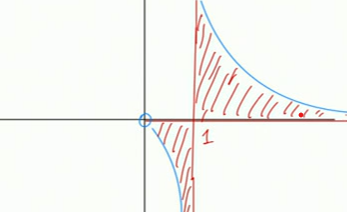
\includegraphics[scale=1.3]{12025-03-12.png}
               \end{center}
               Qui est une droite vertical avec $x = 1$ entre nos deux droite bleu. Néanmoins les lignes bleu ne sont pas inclus, et comme vu sur l'image l'ensemble tends vers les infinis en $x = 1$ et donc, il n'est ni fermé ni borné. Et la raison pour laquelle ce n'est pas ouvert, la  ligne rouge horizontale et fermé et donc ce n'est pas ouvert.
               \begin{framedremark}
                   Attention à faire attention car ici les courbes bleu impliquent que l'ensemble n'est pas fermé mais même si elles étaient fermés, il manquerait quand même le point $0$ qui impliquerait que l'ensemble ne serait pas fermé.
               \end{framedremark}
       \end{enumerate}
\end{subparag}
\end{parag}

\chapter{Fonction réelles de plusieurs variables réelles limite et continuité}
\subsection{Définition et exemples}
\begin{definition}
    Soit $E \subset \mathbb{R}^n $ sous-ensemble non-vide, $n \geq 1$ Une fonction $f : E \to \mathbb{R}$ est une application qui envoie chaque point $ \overline{x} = (x_1, \dots, x_n) \in E$ dans $ \mathbb{R}$. \\
    $E$ est le domaine de définition de $f$ et $f(E)\subset \mathbb{R}$ est l'ensemble image.
\end{definition}
\begin{parag}{Exemple 1}
    \begin{align*}
        f(x, y) = \sqrt{1 - (x^2 - y^2)}
    \end{align*}
    
    
\end{parag}
\begin{parag}{Exemple 2}
    \begin{align*}
        f(x, y) = 2x + 1
    \end{align*}
    Plus généralement:
    \begin{align*}
        f(x, y) = ax + by + c; \; a, b, c, \in \mathbb{R}, E = \mathbb{R}^2
    \end{align*}
  Comment visualiser cette fonction?\\
  \begin{align*}
      \text{Soit } c = 0
  \end{align*}
  Considérons $f(x, y) = ax + by$: Graphique $F = \{(x, y, z): ax + by = z\} = \{(x, y, z) \in \mathbb{R}^3: ax + by -z = 0\} = \{ (x, y, z) \in \mathbb{R}^3: <(x, y, z), (a, b, -1)> = 0\}$ On a donc un plan dont les valeur $a$, $b$ $-1$ sont les composantes d'un vecteur orthogonal: $ \overline{n} = (a, b, -1)$ et contenant $(0, 0, 0)$.
  \\
  Soit $c \in \mathbb{R}$ arbitraire, alors il faut monter le plan par $c$ unité le long de l'axe $z$ pour obtenir le graphique de $f(x, y) = ax+ by + c$ Et donc:
  \begin{align*}
      z = ax + by + x
  \end{align*}
  qui est le plan $ \perp \overline{n} = (a, b, -1)$ qui contient $(0, 0, c)$
  
  
    
\end{parag}
\begin{parag}{Niveau}
    \begin{definition}
        Soit $f : E \to \mathbb{R}$ et $c \in f(E)$ Alors $ \mathcal{N}_f(c) = \{ \overline{x} \in E: f( \overline{x}) = c\} \subset E$
    \end{definition}
    \begin{subparag}{Exemple 4}
        \begin{align*}
            f(x, y) &= \sin(x^2 + y) : E = \mathbb{R}^2\\
            f(E) &= [-1, 1]
        \end{align*}
        
        \begin{framedremark}
            Je conseil de taper sur google les fonctions pour avoir une bonne visualisation de ces fonctions:
            \begin{center}
                \href{https://www.google.com/search?q=sin(x%5E2+%2B+y)&oq=sin(x%5E2+%2B+y)&gs_lcrp=EgZjaHJvbWUyBggAEEUYOTIICAEQABgWGB4yCAgCEAAYFhgeMggIAxAAGBYYHjIICAQQABgWGB4yCAgFEAAYFhgeMgYIBhBFGDwyBggHEEUYPNIBCDM0MDlqMGo0qAIAsAIB&sourceid=chrome&ie=UTF-8}{google.com}
            \end{center}
            
        \end{framedremark}
        On cherche donc les niveaus:
        \begin{align*}
            \mathcal{N}_f(1) &= \{x, y) \in \mathbb{R}^2: \sin(x^2 + y) = 1\}  \\
                             &= \{(x, y) \in \mathbb{R}^2: x^2 + y = \frac{\pi}{2} + 2k\pi, k \in \mathbb{Z}\}\\
                             &= \{(x, y) \in \mathbb{R}^2: y = -x^2 + \frac{\pi}{2} + 2k\pi, k \in \mathbb{Z}
        \end{align*}
        
        
    \end{subparag}

\end{parag}




















